\newpage
\section{Introductory analyses}
\subsection{Patch Test}
\begin{flushleft}
  \textbf{Inputfile:}
  \ttt{\ttilde/hiqlab/models/tutorial/patch\_test}\\
  \textbf{Lua features introduced:}
  \ttt{make\_material\_e, add\_node, add\_element, set\_bc} \\
  \textbf{MATLAB features introduced:}
  \ttt{Mesh\_load, static\_state, plotmesh, plotfield2d}
\end{flushleft}

The first example introduces the basic commands 
that are used to define the Lua mesh input file
and basic MATLAB commands to conduct static mechanical 
analysis. Since the functions that were introduced in Section ??
of the User's Manual are explained in detail, the
user is strongly recommended to thoroughly understand
this example.

A 10-by-10 square rectangle consisting of 4 bilinear 
quadrilateral elements shown in Figure \ref{fig:PatchTestMesh}
is analyzed. The displacement boundary conditions applied are
zero $x$ displacements on the left edge nodes
with zero $y$ displacement on the left bottom corner node.
A force boundary condition in the $x$ direction is applied on 
the right edge nodes, a value of 2.5 on the corner nodes and 
5.0 at the midside. 

\begin{figure}[htbp]
  \centering
  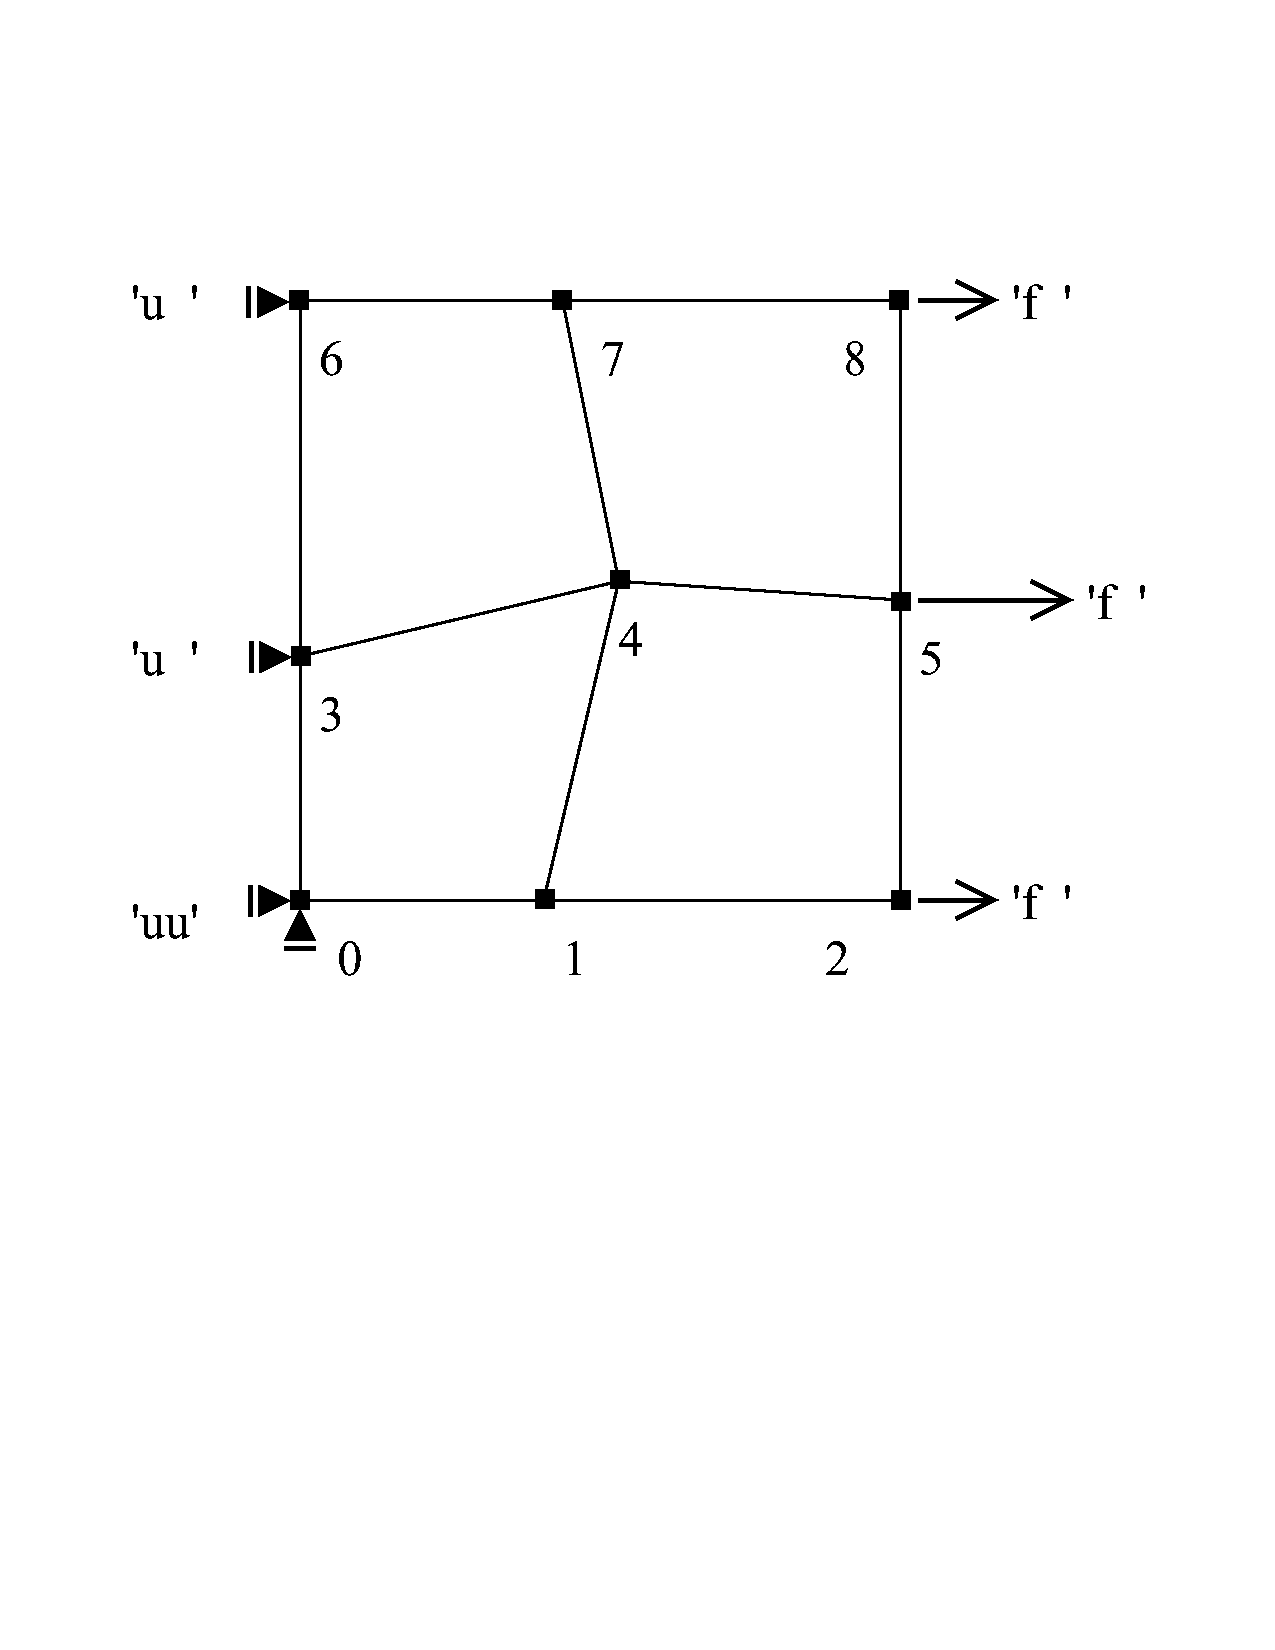
\includegraphics[trim = 0mm 10cm 0mm 1cm, clip, height=8cm]{fig/patchtest.pdf}
  \caption{Patch Test Mesh}
  \label{fig:PatchTestMesh}
\end{figure}

This linear elastic problem is solved under
plane strain assumptions. The material parameters
selected are the following: Youngs's modulus (E)
1000, Poisson ratio (nu) 0.25. The exact solution 
is given as,
\begin{eqnarray}
  u = 0.009375x; ~~ v=-0.003125y \nonumber
\end{eqnarray} 
and stresses are,
\begin{eqnarray}
  \sigma_{xx} = 1.0;~~\sigma_{yy} = 0.0;~~
  \sigma_{xy} = 0.0;~~\sigma_{zz} = 0.25~. \nonumber
\end{eqnarray}

\clearpage
\subsubsection*{Input file (LUA)}
\begin{flushleft}
  \textbf{Inputfile:}
  \ttt{\ttilde/hiqlab/models/tutorial/patch\_test/patch\_test.lua}\\
\end{flushleft}
\hspace{1in}
{\footnotesize
\listinginput[10]{1}{../../../models/tutorial/patch_test/patch_test.lua}
}

\clearpage
\begin{itemize}

  \item{\textbf{Include function definition file:}}
  To use the predefined functions, the definition files
  must be included throught the command \ttt{require}.
  (See section on \ttt{require} command and file \ttt{common.lua}
  for further details).

  \item{\textbf{Construct mesh:}}
  The first line defines and constructs 
  a new \ttt{Mesh} object, where the
  argument "2" defines the physical dimension of
  the mesh ( x,y coordinates). The assignment to 
  {\tt mesh}, passes a reference to the variable.

  \item{\textbf{Construct element:}}
  First a material table \ttt{mtype} is defined. The
  required fields for a static mechanical problem are 
  the Youngs modulus \ttt{E} and Poisson ration \ttt{nu}.
  This material type, along with the string defining the 
  type of analysis is given to the command \ttt{make\_material\_e}
  which produces an elastic material named \ttt{etype}
  \begin{verbatim}
      etype = make_material_e( mtype, 'planestrain');
  \end{verbatim}
  This element is used when elements are added to the \ttt{mesh}.

  \item{\textbf{Define nodal coordinates and element connectivity:}}
  The following two portions of code define arrays of nodal 
  coordinates and element connectivity. The array \ttt{x}
  stores the x and y coordinates of each node consecutively.
  The array \ttt{con} stores the connectivity
  of each element consecutively. In this case, each set of 4 numbers 
  correspond to the connectivity of each 4-noded bilinear 
  quadrilateral element in the mesh. The order of the node 
  numbering for each quadrilateral is defined as fixing the x
  direction first and sweeping across y. For details on this
  see the section on node numbering for elements in the User's
  manual.
  The numbering of the nodes in Lua is zeros based, coinciding
  with that of C++.
  (See section on Mesh Description of the User's manual for details).

  \item{\textbf{Assign nodes and elements to the mesh:}}
  Nodes and elements are assigned to the mesh by the commands
  \ttt{add\_node} and \ttt{add\_element}. The
  array \ttt{x} with 9 nodes and 
  4 bilinear quadrilateral elements of \ttt{etype} with
  connectivity defined n {\tt con} are added to the mesh.

  \item{\textbf{Define and assign boundary conditions:}}
  Boundary conditions in Lua are defined by functions. Depending
  on the physical dimension of the mesh it takes from 1 (x coordinate)
  to 3 (x,y,z coordinate) arguments. The function should output 
  a string defining the boundary condition and numerical values.
  \ttt{u} denotes a fixed boundary condition, \ttt{f} denotes a 
  forced boundary condition, and a blank denotes that no boundary
  condition will be applied. (See Section on Mesh Description of
  User's manual for details. See Section on Helper Lua function for
  mesh for details on mesheq). The mapping between nodal degrees
  of freedom and order of these slots depends on the order in
  which the elements which link the degrees of freedom are 
  added. 

  Once the boundary condition function defined, it is assigned 
  to the mesh through the \ttt{set\_bc} command.

\end{itemize}

\clearpage
\subsubsection*{Solve static problem (MATLAB)}
\begin{flushleft}
  \textbf{Inputfile:}
  \ttt{\ttilde/hiqlab/models/tutorial/patch\_test/patch\_test.m}\\
\end{flushleft}
\hspace{1in}
{\footnotesize
\listinginput[10]{1}{../../../models/tutorial/patch_test/patch_test.m}
}

\clearpage
Once the mesh is defined, the next step is to solve the problem.
This can be done both in Lua and MATLAB. Here we present the MATLAB
interface. 

\begin{itemize}

  \item{\textbf{Load input file}}
  First the Lua mesh input file must be loaded.
  This is conducted by the \ttt{Mesh\_load} command
  which returns a reference to the \ttt{mesh} object 
  and a reference to the variables in the Lua file. 
  One can interact with the Lua input file through 
  this handle \ttt{L}.

  \item{\textbf{View mesh}}
  The mesh can be viewed with the \ttt{plotmesh} command. 
  An optional structure \ttt{opt} can be passed as
  an argument for several options. In this case the
  axis equal feature is activated. 
  The mesh plot for this example
  is shown in Figure \ref{fig:PatchTestMeshMATLAB}. The
  nodes with displacement boundary conditions have a green cross,
  and the nodes with forced boundary conditions have a red cross
  overlayed. 

  \item{\textbf{Solve static problem}}
  The stiffness matrix and forcing vectors are formed and
  and solved for the displacements by the \ttt{static\_state}
  function. The residual of the equilibrium equations is 
  defined as,
  \begin{eqnarray}
  R(u) &=& P(u) - F
  \end{eqnarray}
  where $F$ is the vector of applied forces, $u$
  is the vector of displacments, and for a static
  linear elastic problem $P$ is defined as,
  \begin{eqnarray}
  P   &=& K u~~.
  \end{eqnarray}
  \ttt{static\_state} solves this equation in both the
  linear case and nonlinear case. To invoke the nonlinear 
  case an option must be passed.

  \item{\textbf{Display results}}
  The displacements can be visualized by the command 
  \ttt{plotfield2d}.
  An optional structure \ttt{opt} can be passed as
  an argument for several options. In this case the
  the displacements are magnified 10 times in the 
  visualization.  
  The $x,y$ displacements for this example
  are shown in Figure \ref{fig:PatchTestDisplacements}. The
  top figure shows the $x$ displacements and the bottom shows
  the $y$ displacements. The colors represent the magnitude
  of the displacements, red for positive and blue for negative
  displacements.

\end{itemize}

\begin{figure}[htbp]
  \begin{minipage}{0.45\linewidth}
    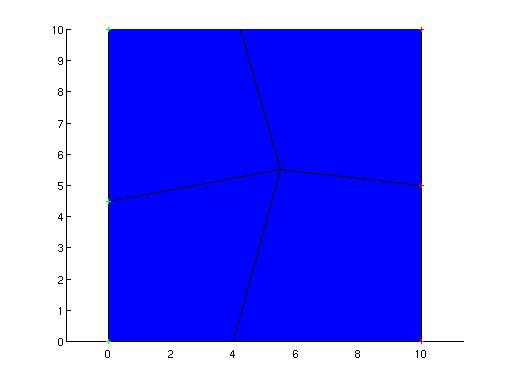
\includegraphics[width=\linewidth]{fig/patch_test_mesh_matlab.jpg}
    \caption{Patch Test Mesh from MATLAB}
    \label{fig:PatchTestMeshMATLAB}
  \end{minipage}
  \hfill
  \begin{minipage}{0.45\linewidth}
    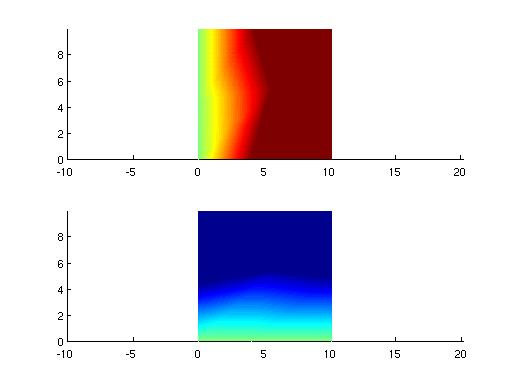
\includegraphics[width=\linewidth]{fig/patch_test_disp_matlab.jpg}
    \caption{Patch Test Displacements}
    \label{fig:PatchTestDisplacements}
  \end{minipage}
\end{figure}

\clearpage
\subsection{2D Cantilever Beam}
\begin{flushleft}
  \textbf{Inputfile:}
  \ttt{\ttilde/hiqlab/models/tutorial/cantilever\_beam}\\
  \textbf{Lua features introduced:}
  \ttt{blocks2d, blocks2dn, mesheq, order, dense}\\
  \textbf{MATLAB features introduced:}
\end{flushleft}
Here we present the analysis of a cantilever beam subjected
to a point load at the end. This example exhibits
the easy to use block commands to define the mesh, as well as 
global parameters that are used for convenience. 

The 10-by-2 2D cantilever beam in Figure \ref{fig:CantileverBeam}, 
which is fixed on the left end and has a unit force applied at the 
right end, is analyzed. 
\begin{figure}[htbp]
  \centering
  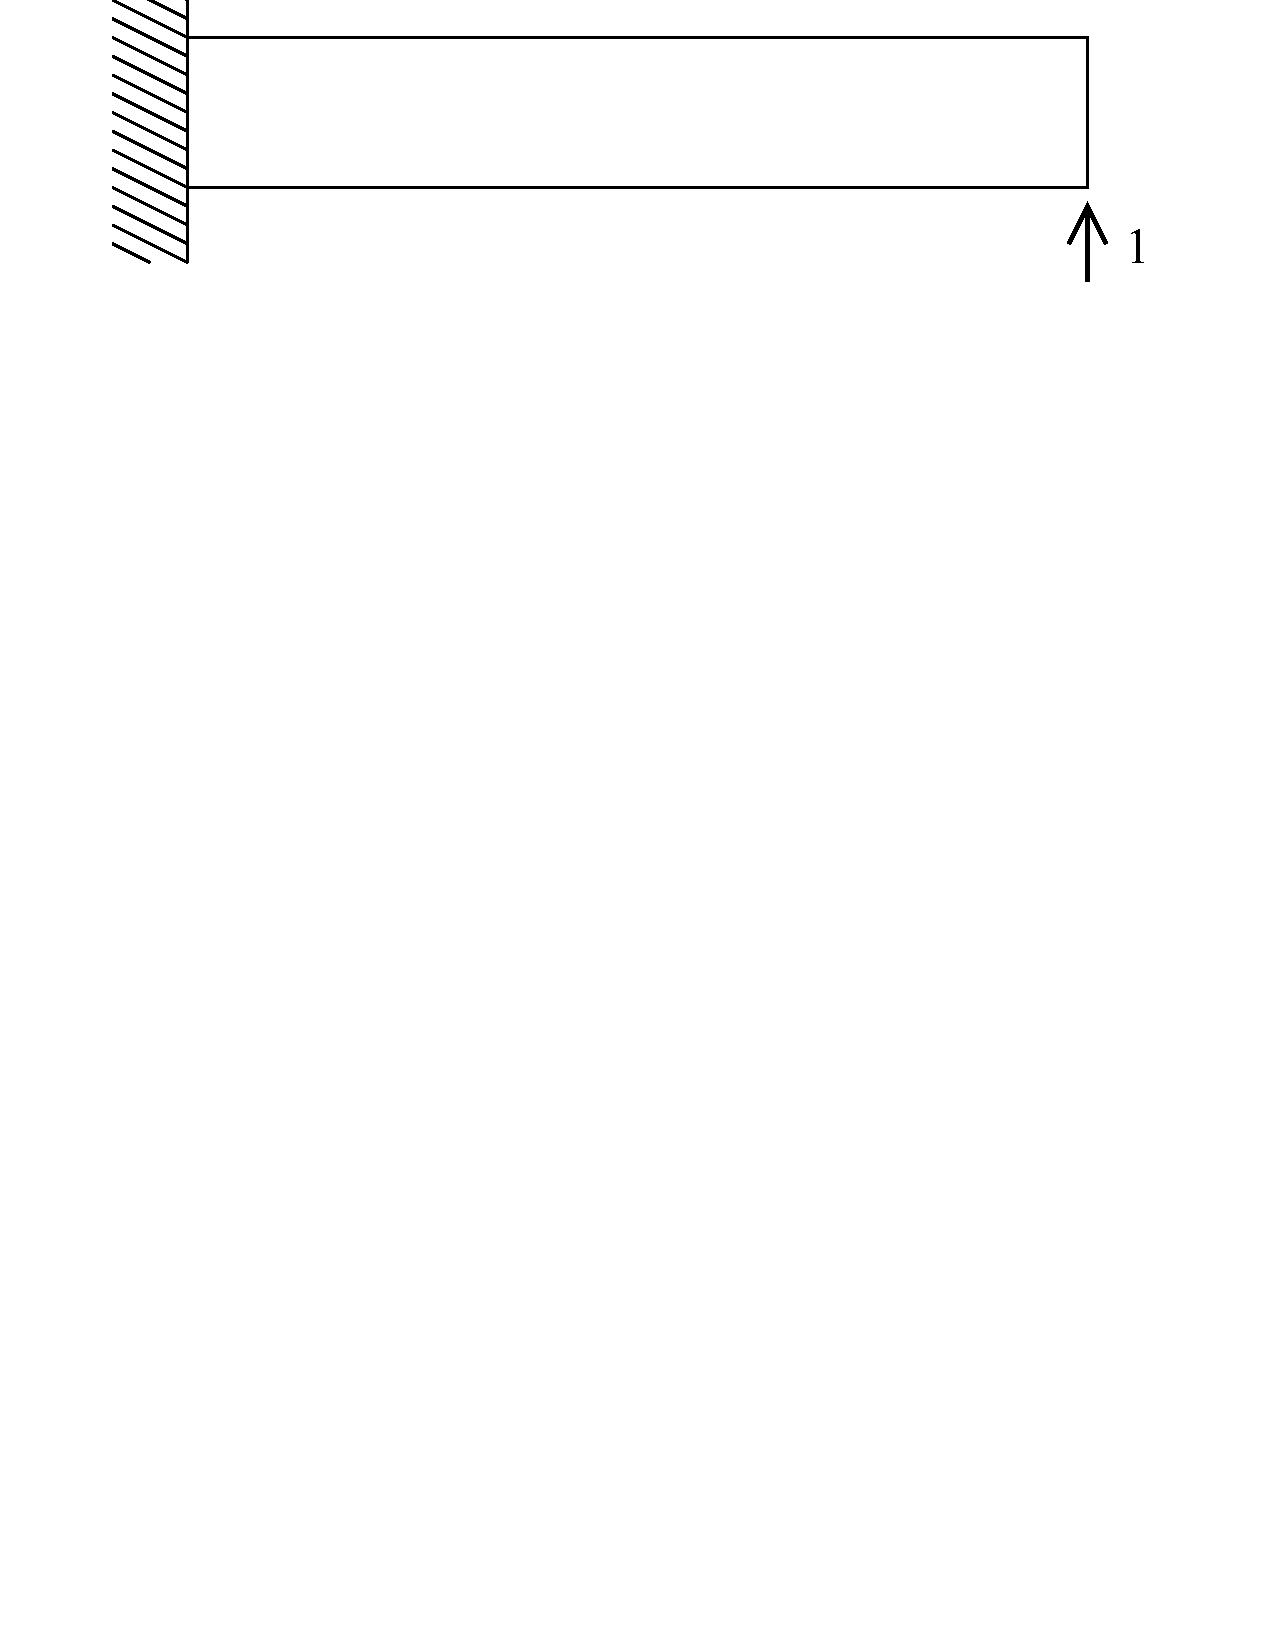
\includegraphics[trim = 0mm 9in 0mm 0cm, clip, height=1in]{fig/cantileverbeam.pdf}
  \caption{Cantilever Beam}
  \label{fig:CantileverBeam}
\end{figure}

Three different Lua mesh input files are presented to solve 
the same problem.
\begin{enumerate}

  \item{\ttt{beam\_test.lua}}: Uses standard \ttt{add\_nodes} and
  \ttt{add\_elements} commands to construct mesh.

  \item{\ttt{beam\_test\_blocks2dn.lua}}: Uses the \ttt{add\_blocks2dn}
  command to construct mesh.

  \item{\ttt{beam\_test\_blocks2d.lua}}: Uses the \ttt{add\_blocks2d}
  command to construct mesh.

\end{enumerate}
The first file is presented to express the tedium involved in
using the \ttt{add\_nodes} and \ttt{add\_elements} command when
the number of nodes and elements increases. This tedium can be 
avoided by using the block generators that are available. The
latter two files use two of these to generate the mesh. All
three files use the same MATLAB file to execute,
\begin{enumerate}
  \item{\ttt{beam\_test.m}}
\end{enumerate}
since only the Lua mesh input file differ. 

\clearpage

\subsubsection*{Input file (LUA)}
\begin{flushleft}
  \textbf{Inputfile:}
  \ttt{\ttilde/hiqlab/models/tutorial/cantilever\_beam/beam\_test.lua}\\
  \ttt{\ttilde/hiqlab/models/tutorial/cantilever\_beam/beam\_test\_blocks2dn.lua}\\
  \ttt{\ttilde/hiqlab/models/tutorial/cantilever\_beam/beam\_test\_blocks2d.lua}\\
\end{flushleft}
\hspace{1in}
\begin{figure}[htbp]
  {\footnotesize
  \listinginput[10]{1}{lua/beam_test_mutual.lua.tex}
  }
  \caption{Matching part of Lua Input file for cantilever beam}
  \label{fig:LuaFile:beam_test_mutual.lua}
\end{figure}

\clearpage
Figure \ref{fig:LuaFile:beam_test_mutual.lua} is the
part of the Lua file that overlap within the three input
files. The portion 'Define nodes and elements' and 
'Add nodes and elements to mesh' differs between the three files. 

\begin{itemize}

  \item{\textbf{Include function definition file:}}
  To use the predefined functions, the definition files
  must be included throught the command \ttt{require}.
  (See section on \ttt{require} command and file \ttt{common.lua}
  for further details).

  \item{\textbf{Construct mesh:}}
  The first line defines and constructs 
  a new \ttt{Mesh} object, where the
  argument "2" defines the physical dimension of
  the mesh ( x,y coordinates). The assignment to 
  \ttt{mesh}, passes a reference to the variable.

  \item{\textbf{Construct element:}}
  First a material table \ttt{mtype} is defined. The
  required fields for a static mechanical problem are 
  the Youngs modulus \ttt{E} and Poisson ration \ttt{nu}.
  This material type, along with the string defining the 
  type of analysis is given to the command \ttt{make\_material\_e}
  which produces an elastic material named \ttt{etype}.
  \begin{verbatim}
      etype = make_material_e( mtype, 'planestrain');
  \end{verbatim}
  This element is used when elements are added to the \ttt{mesh}.

  \item{\textbf{Define nodal coordinates and element connectivity:}}
  \item{\textbf{Assign nodes and elements to the mesh:}}
  This portion of the code differs between the three files.
  Each code generate a beam with 8 quadrilateral bilinear 
  elements, but the amount of code required to define this
  greatly differ. What should be emphasized is the short
  amount of code required when block generators are used.
  (See section on block generators for more details).

  In each case \ttt{div\_x, div\_y} define the number of 
  elements along the $x,y$ direction, \ttt{order} defines the
  order of the elements to be used which is in this case one(linear),
  \ttt{dense\_x,dense\_y} define the approximate size of an 
  element. 
  \begin{enumerate}

    \item{\ttt{beam\_test.lua}}
    Uses standard for loops to define the nodal array \ttt{x} and
    connectivity array \ttt{con}, and then adds these to the 
    mesh through the commands \ttt{add\_node} and \ttt{add\_element}.
    Due to the various indices, this code is error prone. 

    \item{\ttt{beam\_test\_blocks2dn.lua}}
    Uses the \ttt{add\_blocks2d} command to define a block of 
    elements with linear order. The block is defined to have 
    \ttt{div\_x+1=5} nodes along the $x$ direction and 
    \ttt{div\_y+1=3} nodes along the $y$ direction.

    \item{\ttt{beam\_test\_blocks2d.lua}}
    Uses the \ttt{add\_blocks2d} command to define a block of 
    elements with linear order. The block is defined to have 
    \ttt{div\_x+1=5} nodes along the $x$ direction and 
    \ttt{div\_y+1=3} nodes along the $y$ direction.
  \end{enumerate}

  \item{\textbf{Define and assign boundary conditions:}}
  Boundary conditions in Lua are defined by functions. Depending
  on the physical dimension of the mesh it takes from 1 (x coordinate)
  to 3 (x,y,z coordinate) arguments. The function should output 
  a string defining the boundary condition and numerical values.
  \ttt{u} denotes a fixed boundary condition, \ttt{f} denotes a 
  forced boundary condition, and a blank denotes that no boundary
  condition will be applied. (See Section on Mesh Description of
  User's manual for details. See Section on Helper Lua function for
  mesh for details on mesheq).

  Once the boundary condition function defined, it is assigned 
  to the mesh through the \ttt{set\_bc} command.

\end{itemize}


\clearpage
\begin{figure}[htbp]
  {\footnotesize
  \listinginput[10]{1}{lua/beam_test_orig.lua.tex}
  }
  \caption{Differing part of Lua Input file for cantilever 
                                     beam(\ttt{beam\_test.lua})}
  \label{fig:LuaFile:beam_test.lua}
%\end{figure}
%\begin{figure}[htbp]
  {\footnotesize
  \listinginput[10]{1}{lua/beam_test_blocks2dn.lua.tex}
  }
  \caption{Differing part of Lua Input file for cantilever 
                         beam(\ttt{beam\_test\_blocks2dn.lua})}
  \label{fig:LuaFile:beam_test_blocks2dn.lua}
%\end{figure}
%\begin{figure}[htbp]
  {\footnotesize
  \listinginput[10]{1}{lua/beam_test_blocks2d.lua.tex}
  }
  \caption{Differing part of Lua Input file for cantilever 
                         beam(\ttt{beam\_test\_blocks2d.lua})}
  \label{fig:LuaFile:beam_test_blocks2d.lua}
\end{figure}

\clearpage
\subsubsection*{Solve static problem (MATLAB)}
\begin{flushleft}
  \textbf{Inputfile:}
  \ttt{\ttilde/hiqlab/models/tutorial/cantilever\_beam/beam\_test.m}\\
\end{flushleft}
\hspace{1in}
{\footnotesize
\listinginput[10]{1}{../../../models/tutorial/cantilever_beam/beam_test.m}
}
Once the mesh is defined, the next step is to solve the problem.
This can be done both in Lua and MATLAB. Here we present the MATLAB
interface. This file is identical
to the patch\_test and we refer to the section for details.
The mesh and displacements are shown in 
Figure \ref{fig:CantileverBeamMeshMATLAB}
and Figure \ref{fig:CantileverBeamDisplacements}.

\begin{figure}[htbp]
  \begin{minipage}{0.45\linewidth}
    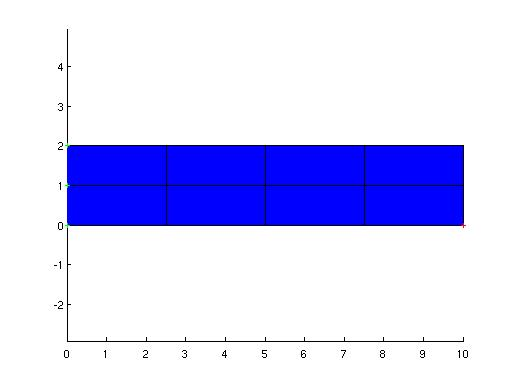
\includegraphics[width=\linewidth]{fig/cantilever_beam_mesh_matlab.jpg}
    \caption{Cantilever Beam mesh from MATLAB}
    \label{fig:CantileverBeamMeshMATLAB}
  \end{minipage}
  \hfill
  \begin{minipage}{0.45\linewidth}
    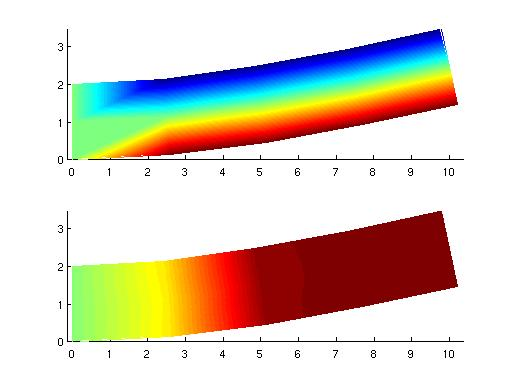
\includegraphics[width=\linewidth]{fig/cantilever_beam_disp_matlab.jpg}
    \caption{Cantilever Beam Displacements}
    \label{fig:CantileverBeamDisplacements}
  \end{minipage}
\end{figure}

\clearpage
\subsection{Circular Disk}
\begin{flushleft}
  \textbf{Inputfile:}
  \ttt{\ttilde/hiqlab/models/tutorial/circular\_disk}\\
  \textbf{Lua features introduced:}
  \ttt{add\_block\_shape, add\_curved\_block\_shape2d, tie, meshtol, or}
  \textbf{MATLAB features introduced:}
  Using params in \ttt{Mesh\_load}
\end{flushleft}
Here we present the analysis of a circular disk subjected
to a point load at the top and bottom. This example exhibits
the easy to use block commands to define the curved meshes,
the ability to pass values into the Lua mesh input file, and 
global parameters that are used for convenience. 

The unit circular disk in Figure \ref{fig:CircularDisk}, which
is 4-fold symmetric is analyzed. Due to this symmetry, only
the quarter in Figure \ref{fig:CircularDiskQuarter} is meshed.
The $y$ displacements of the bottom edge is set to zero, as well as
the $x$ displacements of the left edge. A force of -5 is applied
at the top most node in the $x$ direction. 

In this example, block generators are used  to mesh this disk.
The disk is divided into the 3 parts with corresponding control
nodes shown in Figure \ref{fig:CircularDiskQuarter}.

\begin{figure}[htbp]
  \begin{minipage}{0.45\linewidth}
    \centering
    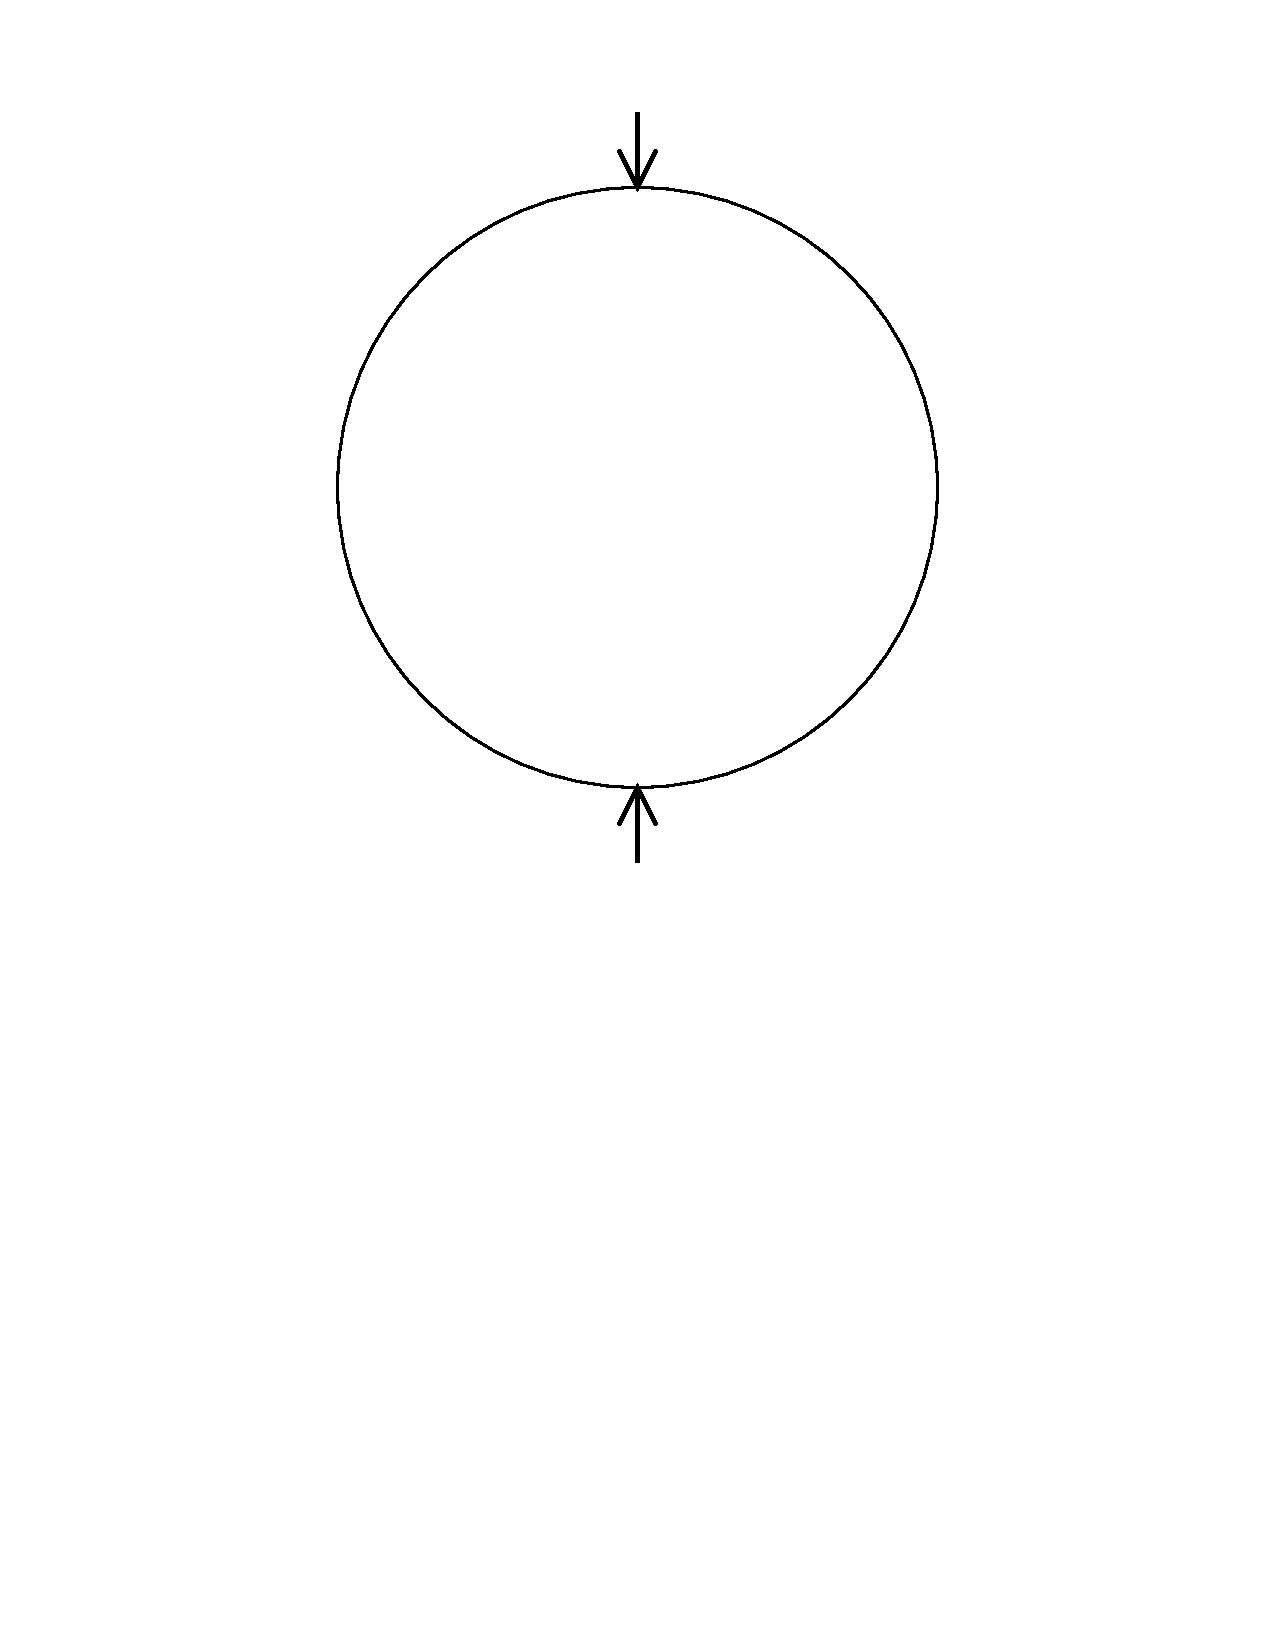
\includegraphics[trim = 1in 5in 1in 0cm, clip, height=2in]{fig/circulardisk.pdf}
    \caption{Circular Disk}
    \label{fig:CircularDisk}
  \end{minipage}
  \begin{minipage}{0.45\linewidth}
    \centering
    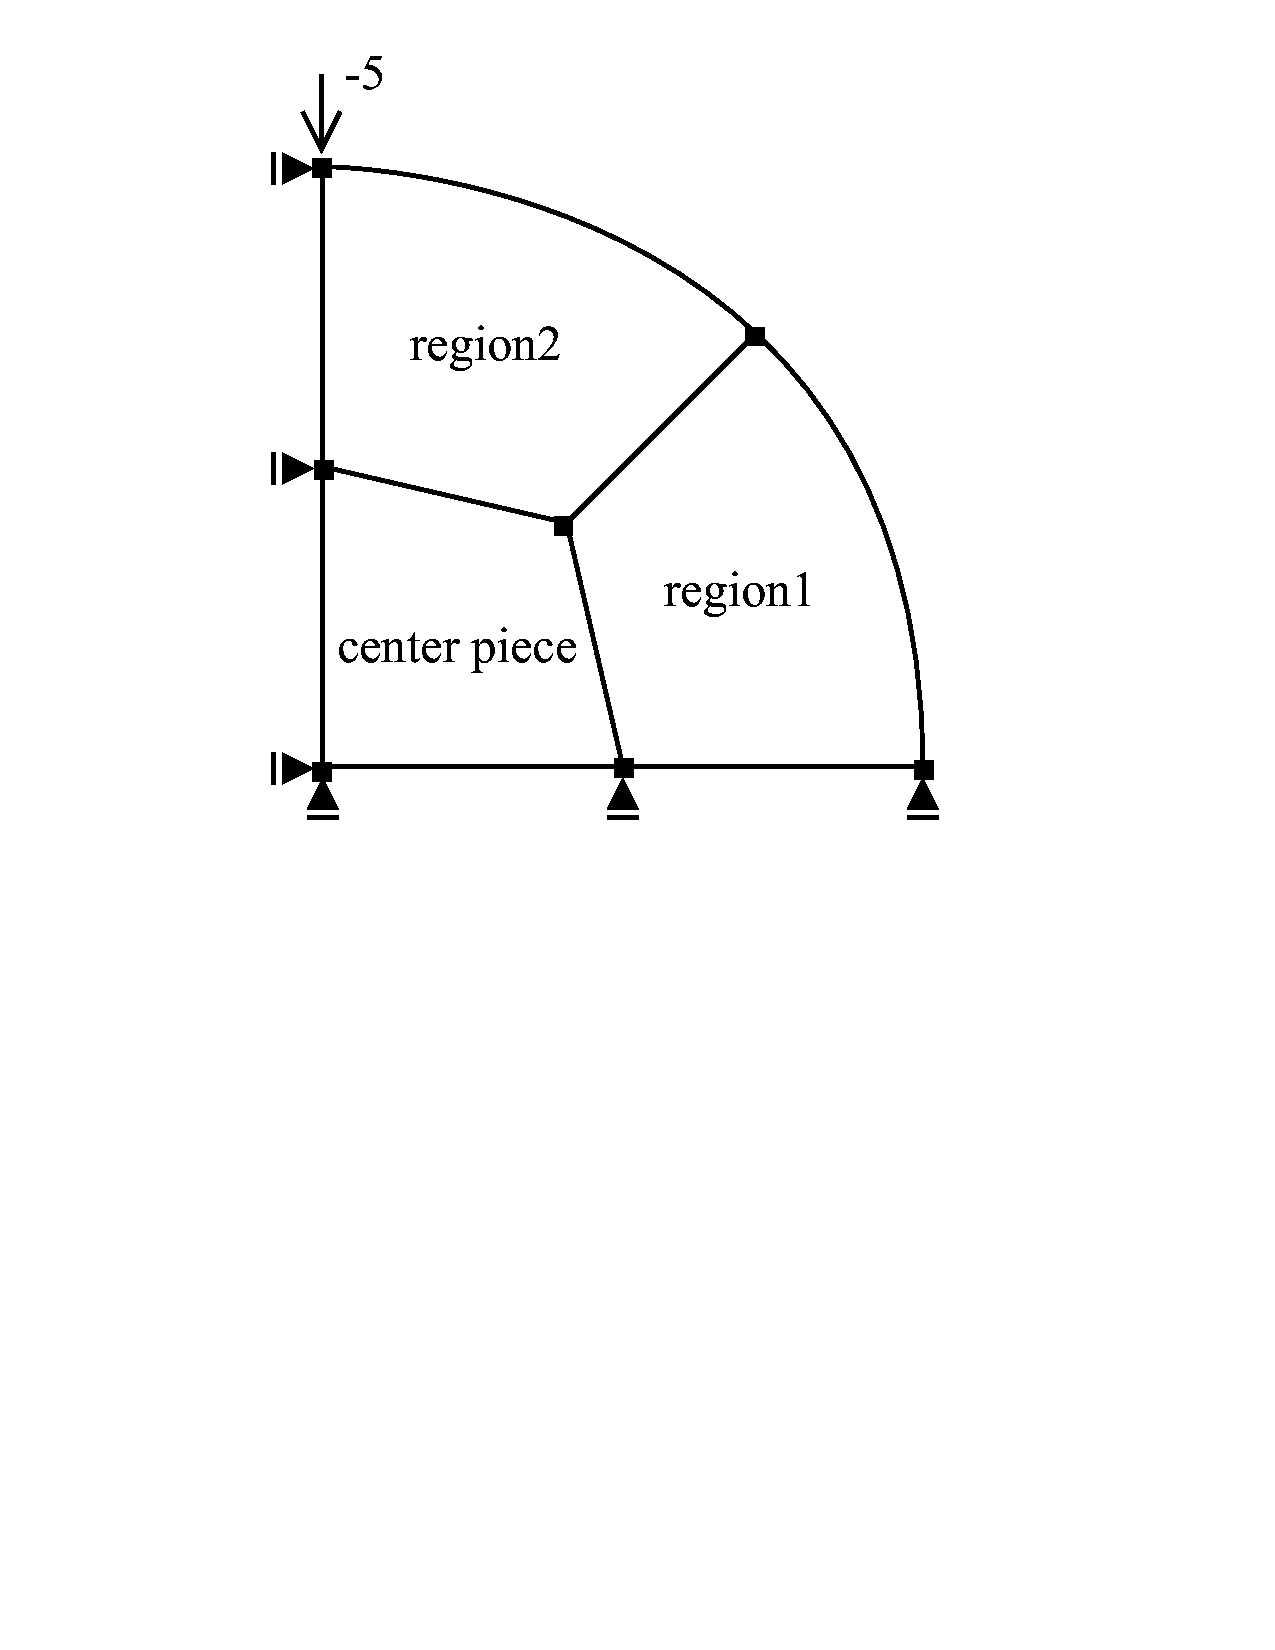
\includegraphics[trim = 0.5in 5in 0.5in 0cm, clip, height=2in]{fig/circulardiskquarter.pdf}
    \caption{Quarter of the Circular Disk}
    \label{fig:CircularDiskQuarter}
  \end{minipage}
\end{figure}

\clearpage
\subsubsection*{Input file (LUA)}
\begin{flushleft}
  \textbf{Inputfile:}
  \ttt{\ttilde/hiqlab/models/tutorial/circular\_disk/circular\_disk.lua}\\
\end{flushleft}
\hspace{1in}
{\footnotesize
\listinginput[10]{1}{../../../models/tutorial/circular_disk/circular_disk.lua}
}

\clearpage
\begin{itemize}

  \item{\textbf{Include function definition file:}}
  To use the predefined functions, the definition files
  must be included throught the command \ttt{require}.
  (See section on \ttt{require} command and file \ttt{common.lua}
  for further details).

  \item{\textbf{Construct mesh:}}
  The first line defines and constructs 
  a new \ttt{Mesh} object, where the
  argument "2" defines the physical dimension of
  the mesh ( x,y coordinates). The assignment to 
  \ttt{mesh}, passes a reference to the variable.

  \item{\textbf{Construct element:}}
  First a material table \ttt{mtype} is defined. The
  required fields for a static mechanical problem are 
  the Youngs modulus \ttt{E} and Poisson ration \ttt{nu}.
  This material type, along with the string defining the 
  type of analysis is given to the command \ttt{make\_material\_e}
  which produces an elastic material.
  \begin{verbatim}
      etype = make_material_e( mtype, 'planestrain');
  \end{verbatim}
  named \ttt{etype}.
  This element is used when elements are added to the \ttt{mesh}.

  \item{\textbf{Define number of elements along the blocks and element order:}}
  \ttt{num\_elem} defines the number of elements that are placed along
  the $x,y$ directions of the 3 blocks, center piece, region1 and region2.
  \ttt{order} defines the order of each of these elements. By defining
  these variables with the \ttt{or} statement, it allows one to pass
  parameters from the running MATLAB environment into the Lua environment.
  If the variables \ttt{num\_elem,order} are not predefined, they are 
  set to 1 respectively. \ttt{div\_x,div\_y} define how many nodes the 
  blocks have along each edge. 

  \item{\textbf{Define mesh tolerance:}}
  When the variable \ttt{meshtol} is defined, functions such as 
  \ttt{tie, mesheq, meshle, meshge, meshbetween} take this as a default
  value when no argument considering tolerance is given. This can be 
  observed in the boundary function definition.

  \item{\textbf{Define nodal coordinates:}}
  The control nodes for the blocks are defined. \ttt{xc} defines the 
  control nodes for the center piece, \ttt{xr1} for region1, and 
  \ttt{xr2} for region2. Since region1 and region2 are curved blocks,
  curved block generators are applied. This function requires that
  the curvature on the 4 edges be defined. These values are stored in
  \ttt{curv1} and \ttt{curv2} respectively. (see section on block
  generators for details).

  \item{\textbf{Define mesh using block command:}}
  \ttt{add\_block\_shape} is used to isoparametrically map a square
  block to mesh the center piece. Region1 and region2 are meshed by
  the \ttt{add\_curved\_block\_shape2d}.

  \item{\textbf{Tie the mesh together:}}
  The three blocks, center piece, region1, and region2 are tied
  together by the \ttt{tie} command. This function ties together 
  nodes that are within a determined tolerance. Since \ttt{meshtol} 
  is predefined, no argument is required.(See section on mesh
  description for details).

  \item{\textbf{Define and assign boundary conditions:}}  
  Boundary conditions in Lua are defined by functions. Depending
  on the physical dimension of the mesh it takes from 1 (x coordinate)
  to 3 (x,y,z coordinate) arguments. The boundary condition for
  this problem requires that the node at (0,1) have fixed $x$ displacement
  of zero and force of $-5$ in the $y$ direction. The first \ttt{return}
  argument corresponds to this condition. The second \ttt{return} argument
  defines the zero $x$ displacement boundary condition for the left edge,
  and the third the zero $y$ displacement boundary condition for the 
  bottom edge. (See Section on Mesh Description of
  User's manual for details. See Section on Helper Lua function for
  mesh for details on mesheq).

  Once the boundary condition function defined, it is assigned 
  to the mesh through the \ttt{set\_bc} command.

\end{itemize}

\clearpage
\subsubsection*{Solve static problem (MATLAB)}
\begin{flushleft}
  \textbf{Inputfile:}
  \ttt{\ttilde/hiqlab/models/tutorial/circular\_disk/circular\_disk.m}\\
\end{flushleft}
\hspace{1in}
{\footnotesize
\listinginput[10]{1}{../../../models/tutorial/circular_disk/circular_disk.m}
}

\clearpage
Once the mesh is defined, the next step is to solve the problem.
This can be done both in Lua and MATLAB. Here we present the MATLAB
interface. 

\begin{itemize}

  \item{\textbf{Pass parameters into Lua file}}
  Variables from Matlab can be passed into the Lua input file
  by the optional \ttt{params} structure. For this problem, the
  variables \ttt{num\_elem} and \ttt{order} are passed. In the
  Lua input file, the \ttt{or} argument makes this possible. 
  By constructing the Lua input file in this manner, parameteric
  studies such as mesh refinement are easily conducted. For this
  problem, the two parameters are varied to show this. 

  \item{\textbf{Load input file}}
  The optional structure \ttt{params} is given as an argument,
  to the function \ttt{Mesh\_load}
  to pass variables into the Lua input file environment.

\end{itemize}

\clearpage
\subsubsection*{Parametric study (MATLAB)}
Parametric study conducted by varying the variable 
\ttt{num\_elem} and \ttt{order} in the structure \ttt{params}
passed into the Lua environment is presented in this
section. The mesh and displacement plot obtained for each case
is shown in the figures.

\begin{figure}[htbp]
  \begin{minipage}{0.45\linewidth}
    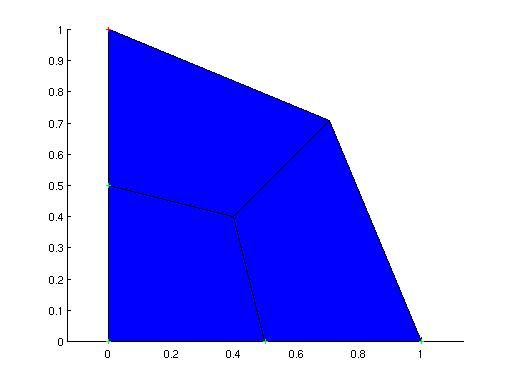
\includegraphics[width=\linewidth]{fig/circular_disk11_mesh_matlab.jpg}
    \caption{Circular Disk mesh from MATLAB(\ttt{num\_elem=1,order=1})}
    \label{fig:CircularDisk11MeshMATLAB}
  \end{minipage}
  \hfill
  \begin{minipage}{0.45\linewidth}
    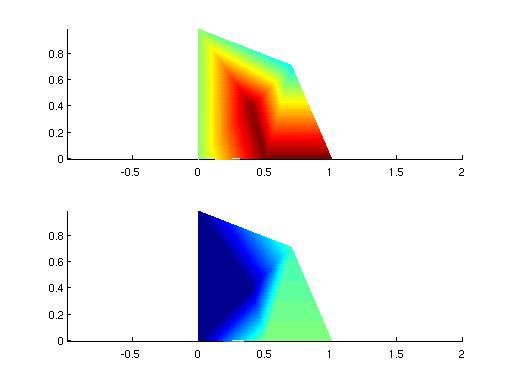
\includegraphics[width=\linewidth]{fig/circular_disk11_disp_matlab.jpg}
    \caption{Circular Disk Displacements(\ttt{num\_elem=1,order=1})}
    \label{fig:CircularDisk11Displacements}
  \end{minipage}
  \begin{minipage}{0.45\linewidth}
    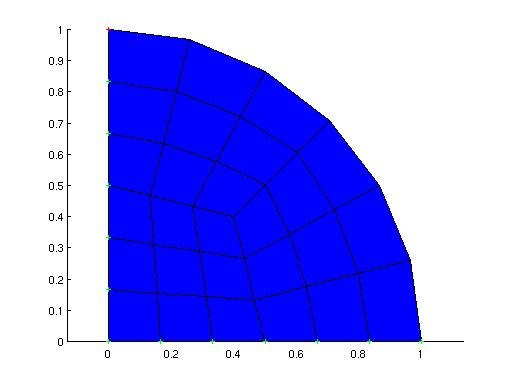
\includegraphics[width=\linewidth]{fig/circular_disk13_mesh_matlab.jpg}
    \caption{Circular Disk mesh from MATLAB(\ttt{num\_elem=1,order=3})}
    \label{fig:CircularDisk13MeshMATLAB}
  \end{minipage}
  \hfill
  \begin{minipage}{0.45\linewidth}
    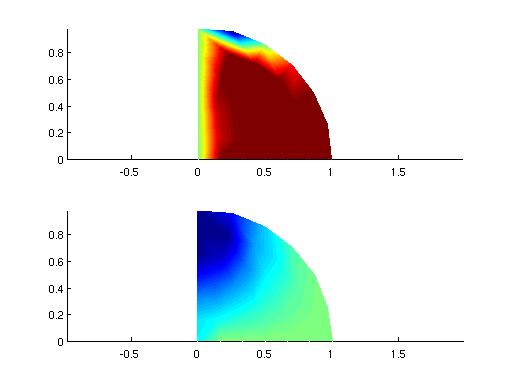
\includegraphics[width=\linewidth]{fig/circular_disk13_disp_matlab.jpg}
    \caption{Circular Disk Displacements(\ttt{num\_elem=1,order=3})}
    \label{fig:CircularDisk13Displacements}
  \end{minipage}
  \begin{minipage}{0.45\linewidth}
    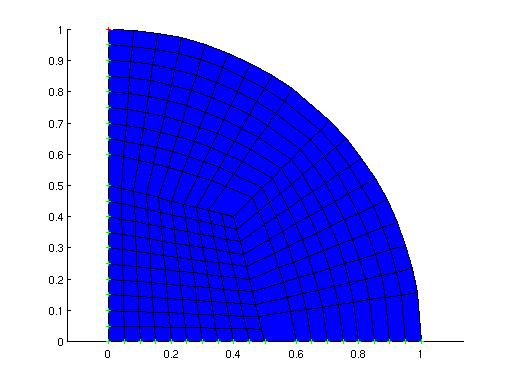
\includegraphics[width=\linewidth]{fig/circular_disk52_mesh_matlab.jpg}
    \caption{Circular Disk mesh from MATLAB(\ttt{num\_elem=5,order=2})}
    \label{fig:CircularDisk52MeshMATLAB}
  \end{minipage}
  \hfill
  \begin{minipage}{0.45\linewidth}
    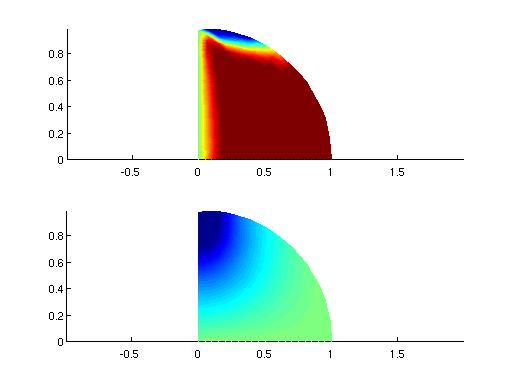
\includegraphics[width=\linewidth]{fig/circular_disk52_disp_matlab.jpg}
    \caption{Circular Disk Displacements(\ttt{num\_elem=5,order=2})}
    \label{fig:CircularDisk52Displacements}
  \end{minipage}
\end{figure}

\clearpage
\subsection{Arch}
\begin{flushleft}
  \textbf{Inputfile:}
  \ttt{\ttilde/hiqlab/models/tutorial/arch}\\
  \textbf{Lua features introduced:}
  \ttt{add\_block\_transform}\\
  \textbf{MATLAB features introduced:}
\end{flushleft}
Here we present the analysis of an arch subjected
to a point load at the top. This example exhibits
the easy to use block commands to define the curved meshes,
the ability to pass values into the Lua mesh input file, and 
global parameters that are used for convenience. 

The arch in Figure \ref{fig:Arch} is analyzed. 
The $x,y$ displacements at the bottom edge is set to zero, and
a force of -5 is applied at the top most node in the $y$ direction. 

In this example, a block generators is used  to mesh this arch.
The control nodes are shown as black squares in  Figure 
\ref{fig:Arch}.

\begin{figure}[htbp]
  \centering
  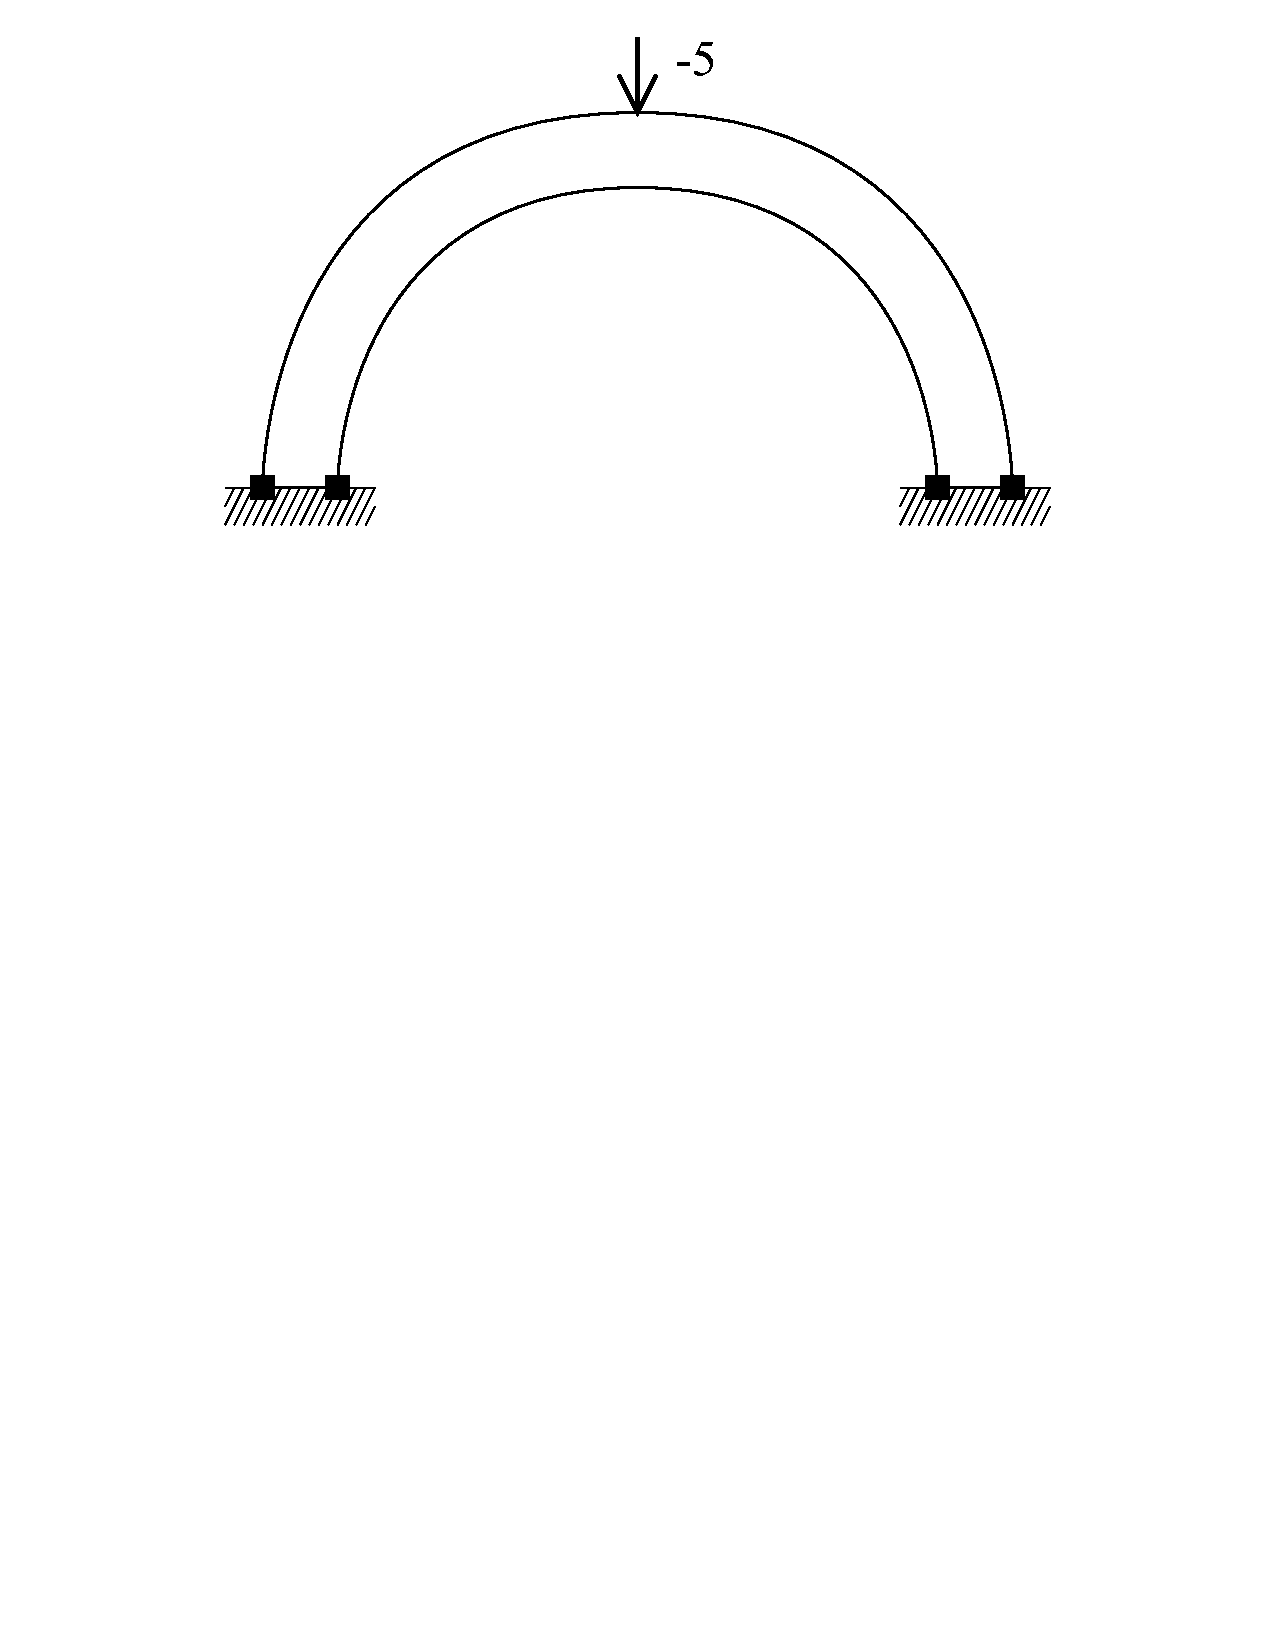
\includegraphics[trim = 1in 5.5in 1in 0cm, clip, height=2in]{fig/arch.pdf}
  \caption{Arch}
  \label{fig:Arch}
\end{figure}

\clearpage
\subsubsection*{Input file (LUA)}
\begin{flushleft}
  \textbf{Inputfile:}
  \ttt{\ttilde/hiqlab/models/tutorial/arch/arch.lua}\\
\end{flushleft}
\hspace{1in}
{\footnotesize
\listinginput[10]{1}{../../../models/tutorial/arch/arch.lua}
}

\clearpage
\begin{itemize}

  \item{\textbf{Define number of elements along the blocks and element order:}}
  \ttt{num\_elem} defines the number of elements that are placed along
  the $y$ directions of the block. The number elements that are placed
  along the $x$ is defined as \ttt{6 num\_elem}.
  \ttt{order} defines the order of each of these elements. By defining
  these variables with the \ttt{or} statement, it allows one to pass
  parameters from the running MATLAB environment into the Lua environment.
  If the variables \ttt{num\_elem,order} are not predefined, they are 
  set to 1 respectively. \ttt{div\_x,div\_y} define how many nodes the 
  blocks have along each edge. 

  \item{\textbf{Define size of arch:}}
  The inner radius of the arch is defined as \ttt{Ri} and the thickness
  by \ttt{Rt}.

  \item{\textbf{Define ring function for block transform:}}
  The function \ttt{ring} which maps a square block to an arch by
  polar coordinate transformation is defined. This function must take
  the $x,y$ coordinates and return new $x,y$ coordinates.

  \item{\textbf{Define mesh using block command:}}
  \ttt{add\_block\_transfor} is used to map a square
  block to an arch by means of polar coordinate transformation.

  \item{\textbf{Define and assign boundary conditions:}}  
  Boundary conditions in Lua are defined by functions. Depending
  on the physical dimension of the mesh it takes from 1 (x coordinate)
  to 3 (x,y,z coordinate) arguments. The boundary condition for
  this problem requires that along the bottom edge the $x,y$ displacements
  are fixed and a force of $-5$ in the $y$ direction at the top node.
  The first \ttt{return} argument corresponds to this condition. 
  The second \ttt{return} argument
  defines the zero $x,y$ displacement boundary condition along the 
  bottom edge.
  (See Section on Mesh Description of
  User's manual for details. See Section on Helper Lua function for
  mesh for details on mesheq).

  Once the boundary condition function defined, it is assigned 
  to the mesh through the \ttt{set\_bc} command.

\end{itemize}

\clearpage
\subsubsection*{Solve static problem (MATLAB)}
\begin{flushleft}
  \textbf{Inputfile:}
  \ttt{\ttilde/hiqlab/models/tutorial/arch/arch.m}\\
\end{flushleft}
\hspace{1in}
{\footnotesize
\listinginput[10]{1}{../../../models/tutorial/arch/arch.m}
}

\clearpage
Once the mesh is defined, the next step is to solve the problem.
This can be done both in Lua and MATLAB. Here we present the MATLAB
interface. 
The mesh and displacement plot obtained for \ttt{node\_num=3,order=2}
is shown in the Figures \ref{fig:Arch32MeshMATLAB} and 
\ref{fig:Arch32Displacements}.

\begin{figure}[htbp]
  \begin{minipage}{0.45\linewidth}
    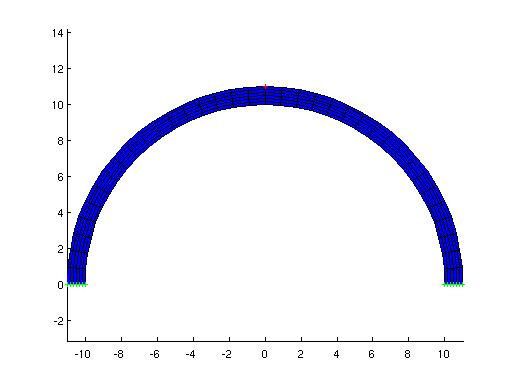
\includegraphics[width=\linewidth]{fig/arch32_mesh_matlab.jpg}
    \caption{Arch mesh from MATLAB (\ttt{num\_elem=3,order=2})}
    \label{fig:Arch32MeshMATLAB}
  \end{minipage}
  \hfill
  \begin{minipage}{0.45\linewidth}
    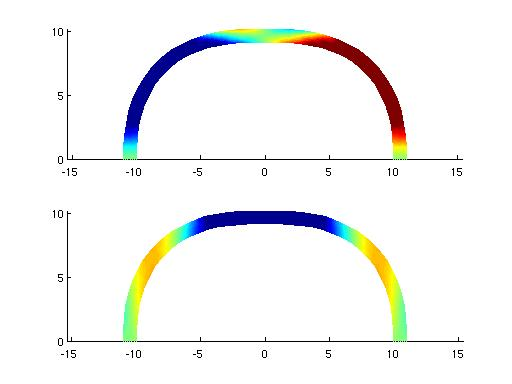
\includegraphics[width=\linewidth]{fig/arch32_disp_matlab.jpg}
    \caption{Arch32 Displacements  (\ttt{num\_elem=3,order=2})}
    \label{fig:Arch32Displacements}
  \end{minipage}
\end{figure}
